\documentclass[cn]{elegantbook}
\usepackage[square,numbers,sort&compress]{natbib}
\newcommand{\upcite}[1]{\textsuperscript{\textsuperscript{\cite{#1}}}}
\usepackage{diagbox}
\usepackage{algorithm}
\usepackage{algorithmicx}
\usepackage{algpseudocode}
\renewcommand{\algorithmicrequire}{\textbf{输入:}}
\renewcommand{\algorithmicensure}{\textbf{输出:}}

\tikzstyle{startstop} = [rectangle, rounded corners, minimum width = 2cm, minimum height=1cm,text centered, draw = black, fill = red!40]
\tikzstyle{arrow} = [->,>=stealth]

% title info
\title{模式识别作业6}
\subtitle{非监督聚类算法}
% bio info
\author{罗雁天}
\institute{清华大学电子系}
\version{2018310742}
\date{\today}
\logo{logo.png}
\cover{cover.jpg}

\begin{document}

\maketitle
\tableofcontents
\mainmatter
\hypersetup{pageanchor=true}
% add preface chapter here if needed
\chapter{Kmeans聚类}
\section{问题描述}
给定数据集``testSet.txt'',包含60行2维数据,每行代表一个样本点,分布如图\ref{intro}所示。
\begin{figure}[!h]
	\centering
	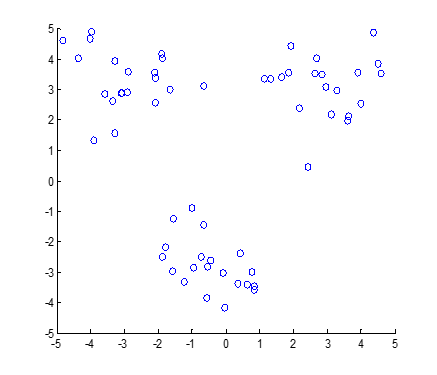
\includegraphics[width=\linewidth]{intro}
	\caption{\label{intro}}
\end{figure}

对这组数据进行kmeans聚类,令$k=2,3,4$。画出聚类结果及每类的中心点,观察聚类结果。记录使用不同初始点时的聚类结果,收敛迭代次数及误差平方和。
\begin{itemize}
	\item $k=3$时,用给出几组初始点进行聚类:
	\begin{itemize}
		\item 初始点组1:[-4.822 4.607;-0.7188 -2.493;4.377 4.864]
		\item 初始点组2:[-3.594 2.857;-0.6595 3.111;3.998 2.519]
		\item 初始点组3:[-0.7188 -2.493;0.8458 -3.59;1.149 3.345]
		\item 初始点组4:[-3.276 1.577;3.275 2.958;4.377 4.864]
	\end{itemize}
	\item $k=2\mbox{或}4$时,自行给出初始点并聚类,观察聚类结果.
\end{itemize}
%\section{算法描述}

\section{实验结果}
\subsection{K=3时}
\paragraph{初始点组1}
使用$\triangle$表示初始聚类中心,$\circ$表示最终聚类中心,不同颜色表示各样本的聚类结果。首先我们采用欧氏距离作为度量,得到实验结果如图\ref{res31}所示。从结果来看,迭代两次便得到了最终的聚类结果,收敛很快。
\begin{figure}[!h]
	\centering
	\begin{minipage}{0.48\linewidth}
		\centering
		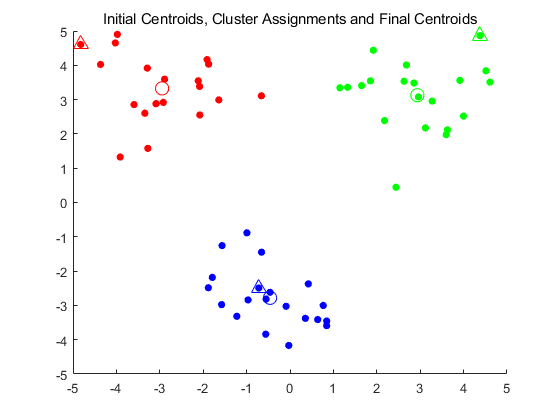
\includegraphics[width=\linewidth]{images/res31}
	\end{minipage}
	\begin{minipage}{0.48\linewidth}
		\centering
		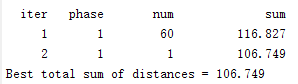
\includegraphics[width=\linewidth]{images/res311}
	\end{minipage}
	\caption{\label{res31}K=3,使用初始点组1聚类结果(欧氏距离作为度量)}
\end{figure}

与之进行对比,我们使用曼哈顿距离作为度量,再次进行实验,结果如图\ref{res311}所示。可以看出,聚类结果有微小的差距,迭代次数同样是2次。由此可以看出,在这种初始化条件下,使用欧氏距离和曼哈顿距离进行Kmeans聚类的结果相近,并且迭代次数都很少,说明这种初始条件效果较好。
\begin{figure}[!h]
	\centering
	\begin{minipage}{0.48\linewidth}
		\centering
		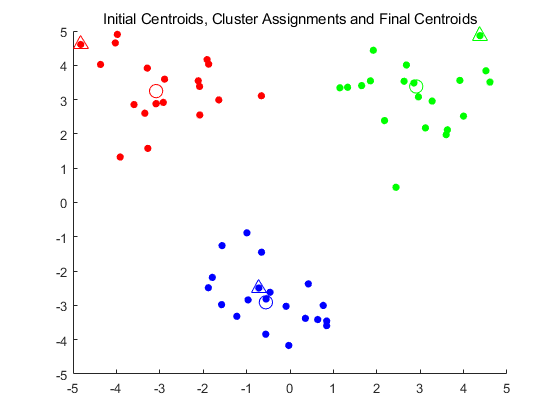
\includegraphics[width=\linewidth]{images/res312}
	\end{minipage}
	\begin{minipage}{0.48\linewidth}
		\centering
		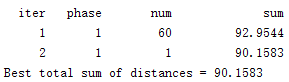
\includegraphics[width=\linewidth]{images/res313}
	\end{minipage}
	\caption{\label{res311}K=3,使用初始点组1聚类结果(曼哈顿距离作为度量)}
\end{figure}

\paragraph{初始点组2}
使用$\triangle$表示初始聚类中心,$\circ$表示最终聚类中心,不同颜色表示各样本的聚类结果。首先我们采用欧氏距离作为度量,得到实验结果如图\ref{res32}所示。从结果来看,迭代两次便得到了最终的聚类结果,收敛很快。
\begin{figure}[!h]
	\centering
	\begin{minipage}{0.48\linewidth}
		\centering
		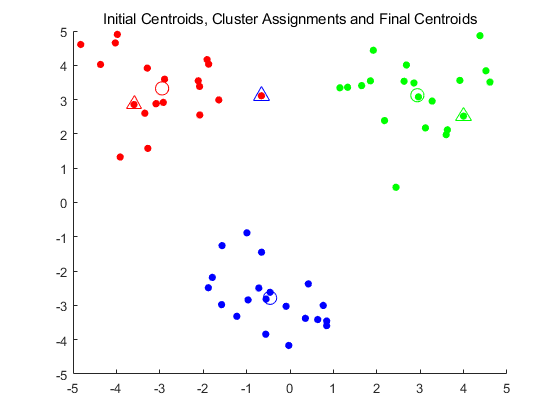
\includegraphics[width=\linewidth]{images/res32}
	\end{minipage}
	\begin{minipage}{0.48\linewidth}
		\centering
		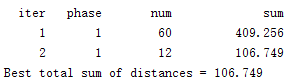
\includegraphics[width=\linewidth]{images/res321}
	\end{minipage}
	\caption{\label{res32}K=3,使用初始点组2聚类结果(欧氏距离作为度量)}
\end{figure}

与之进行对比,我们使用曼哈顿距离作为度量,再次进行实验,结果如图\ref{res321}所示。可以看出,聚类结果有微小的差距,迭代次数同样是2次。由此可以看出,在这种初始化条件下,使用欧氏距离和曼哈顿距离进行Kmeans聚类的结果相近,并且迭代次数都很少。
\begin{figure}[!h]
	\centering
	\begin{minipage}{0.48\linewidth}
		\centering
		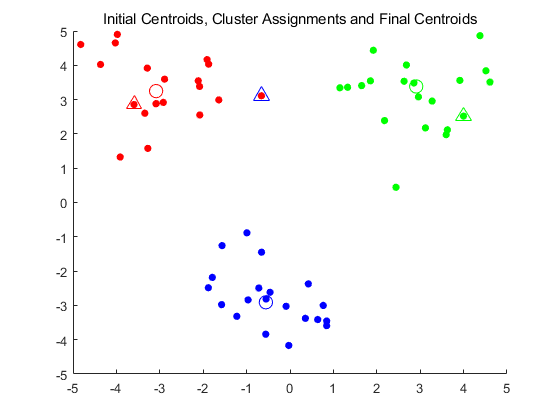
\includegraphics[width=\linewidth]{images/res322}
	\end{minipage}
	\begin{minipage}{0.48\linewidth}
		\centering
		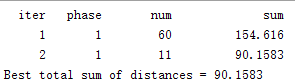
\includegraphics[width=\linewidth]{images/res323}
	\end{minipage}
	\caption{\label{res321}K=3,使用初始点组2聚类结果(曼哈顿距离作为度量)}
\end{figure}

然后我们又尝试使用余弦相似度作为度量进行聚类,结果如图\ref{res322}所示,从结果来看,最后聚类结果还是很不错的,但是迭代次数相比于欧氏距离和曼哈顿距离多了一次,因此在此初始条件下,余弦相似度作为度量的聚类效果不如欧氏距离和曼哈顿距离好。

\begin{figure}[!h]
	\centering
	\begin{minipage}{0.48\linewidth}
		\centering
		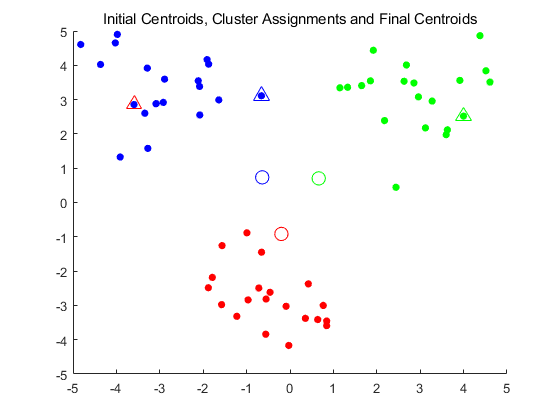
\includegraphics[width=\linewidth]{images/res324}
	\end{minipage}
	\begin{minipage}{0.48\linewidth}
		\centering
		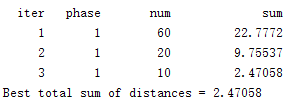
\includegraphics[width=\linewidth]{images/res325}
	\end{minipage}
	\caption{\label{res323}K=3,使用初始点组2聚类结果(余弦相似度作为度量)}
\end{figure}

\paragraph{初始点组3}
同样,使用$\triangle$表示初始聚类中心,$\circ$表示最终聚类中心,不同颜色表示各样本的聚类结果。首先我们采用欧氏距离作为度量,得到实验结果如图\ref{res33}所示。从结果来看,迭代两次便得到了最终的聚类结果,收敛很快,但是聚类结果显然没有之前两组好,由此也可以说明kmeans聚类是初始化敏感的,初始化对最终聚类结果的影响是较大的。
\begin{figure}[!h]
	\centering
	\begin{minipage}{0.48\linewidth}
		\centering
		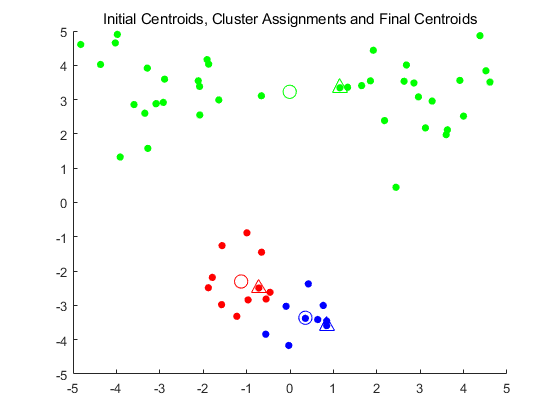
\includegraphics[width=\linewidth]{images/res33}
	\end{minipage}
	\begin{minipage}{0.48\linewidth}
		\centering
		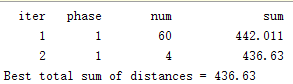
\includegraphics[width=\linewidth]{images/res331}
	\end{minipage}
	\caption{\label{res33}K=3,使用初始点组3聚类结果(欧氏距离作为度量)}
\end{figure}

与之进行对比,我们使用曼哈顿距离作为度量,再次进行实验,结果如图\ref{res331}所示。可以看出,迭代次数是3次,比欧氏距离多了1次,说明收敛较慢。同样,聚类效果相比于之前两组初始条件不好。
\begin{figure}[!h]
	\centering
	\begin{minipage}{0.48\linewidth}
		\centering
		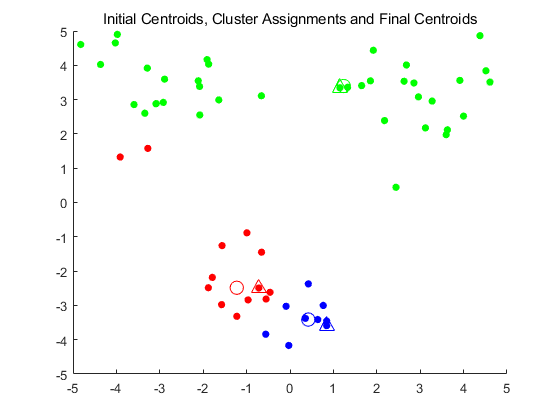
\includegraphics[width=\linewidth]{images/res332}
	\end{minipage}
	\begin{minipage}{0.48\linewidth}
		\centering
		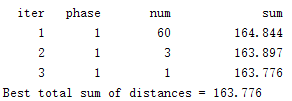
\includegraphics[width=\linewidth]{images/res333}
	\end{minipage}
	\caption{\label{res331}K=3,使用初始点组3聚类结果(曼哈顿距离作为度量)}
\end{figure}

然后我们又尝试使用余弦相似度作为度量进行聚类,结果如图\ref{res332}所示,从结果来看,迭代次数更多了,而且聚类效果也不如之前初始化条件下的好。

\begin{figure}[!h]
	\centering
	\begin{minipage}{0.48\linewidth}
		\centering
		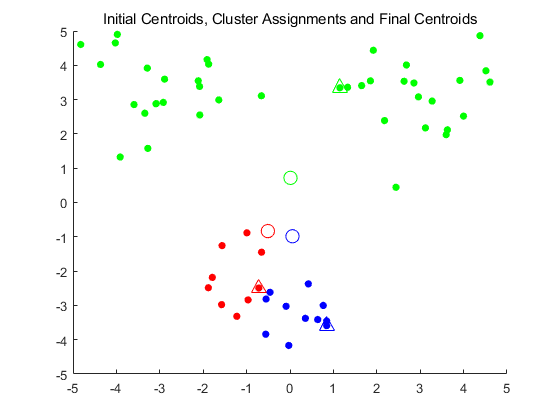
\includegraphics[width=\linewidth]{images/res334}
	\end{minipage}
	\begin{minipage}{0.48\linewidth}
		\centering
		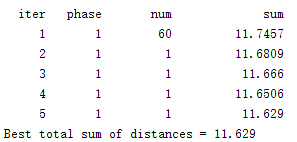
\includegraphics[width=\linewidth]{images/res335}
	\end{minipage}
	\caption{\label{res332}K=3,使用初始点组3聚类结果(余弦相似度作为度量)}
\end{figure}

\paragraph{初始点组4}
使用$\triangle$表示初始聚类中心,$\circ$表示最终聚类中心,不同颜色表示各样本的聚类结果。首先我们采用欧氏距离作为度量,得到实验结果如图\ref{res34}所示。从结果来看,得到的最终结果也没有初始条件1和2的效果好,但是收敛速度还是挺快的。
\begin{figure}[!h]
	\centering
	\begin{minipage}{0.48\linewidth}
		\centering
		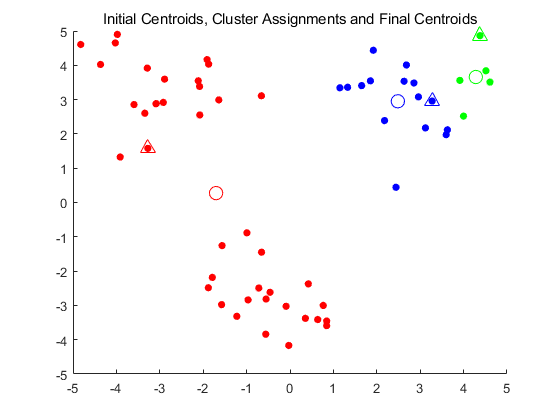
\includegraphics[width=\linewidth]{images/res34}
	\end{minipage}
	\begin{minipage}{0.48\linewidth}
		\centering
		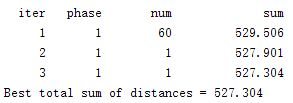
\includegraphics[width=\linewidth]{images/res341}
	\end{minipage}
	\caption{\label{res34}K=3,使用初始点组4聚类结果(欧氏距离作为度量)}
\end{figure}

与之进行对比,我们使用曼哈顿距离作为度量,再次进行实验,结果如图\ref{res341}所示。可以看出,此时的聚类效果和初始条件1和2的类似,比使用欧氏距离得到的结果较好,但是迭代次数稍微多了一点。所以对于此种初始化条件下来看,曼哈顿距离比欧氏距离具有更好的聚类效果。
\begin{figure}[!h]
	\centering
	\begin{minipage}{0.48\linewidth}
		\centering
		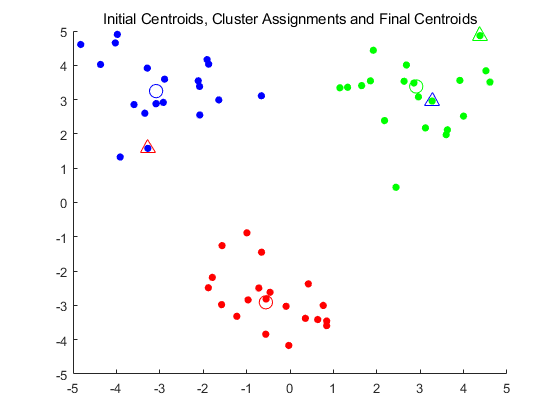
\includegraphics[width=\linewidth]{images/res342}
	\end{minipage}
	\begin{minipage}{0.48\linewidth}
		\centering
		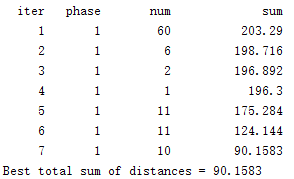
\includegraphics[width=\linewidth]{images/res343}
	\end{minipage}
	\caption{\label{res341}K=3,使用初始点组4聚类结果(曼哈顿距离作为度量)}
\end{figure}

\subsection{K=2}
从之前$K=3$部分的讨论来看,初始的聚类中心对实验结果有较大的影响,因此我们观察数据,设置较好的聚类中心进行实验。并且从之前的讨论来看,使用曼哈顿距离聚类效果更好一些,因此在本部分我们选择曼哈顿距离作为度量。%使用欧氏距离和曼哈顿距离作为度量比余弦相似度效果较好一点,并且在初始聚类中心不好的情况下,曼哈顿距离比欧氏距离聚类效果略好一点,因此在本部分我们选择曼哈顿距离作为度量。

观察数据可以看出,数据主要集中在三部分,要聚类成两类最终结果大概是把其中两类聚在了一起,因此,我们可以构造不同的初始条件,将不同的两类聚类到一起。

\paragraph{初始条件1}
我们选取初始条件为:[-4.822 4.607;4.377 4.864],实验结果如图\ref{res21}所示。从图中可以看出,我们将左上角和下面的两类聚成了一类,右上角聚成了一类。
\begin{figure}[!h]
	\centering
	\begin{minipage}{0.48\linewidth}
		\centering
		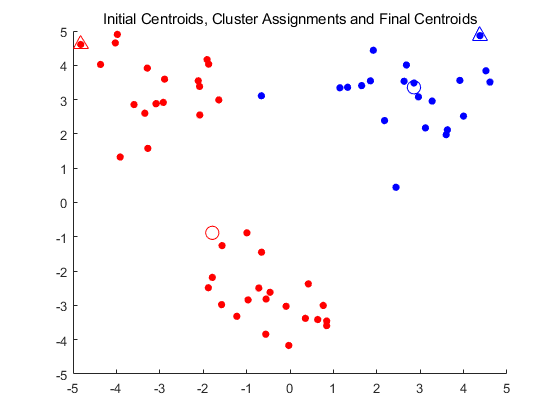
\includegraphics[width=\linewidth]{images/res21}
	\end{minipage}
	\begin{minipage}{0.48\linewidth}
		\centering
		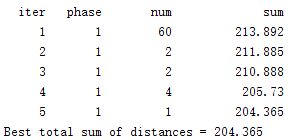
\includegraphics[width=\linewidth]{images/res211}
	\end{minipage}
	\caption{\label{res21}K=2聚类结果(曼哈顿距离作为度量)}
\end{figure}

\paragraph{初始条件2}
我们选取初始条件为:[1.149 3.345;-0.6595 -3.59],实验结果如图\ref{res22}所示。从图中可以看出,我们将左上角和右上角的两类聚成了一类,下面聚成了一类。
\begin{figure}[!h]
	\centering
	\begin{minipage}{0.48\linewidth}
		\centering
		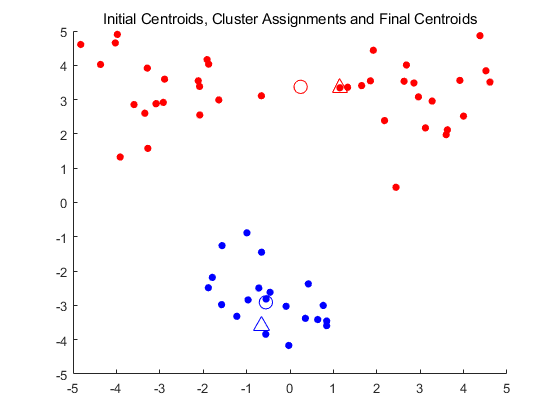
\includegraphics[width=\linewidth]{images/res22}
	\end{minipage}
	\begin{minipage}{0.48\linewidth}
		\centering
		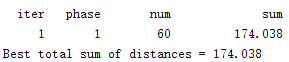
\includegraphics[width=\linewidth]{images/res221}
	\end{minipage}
	\caption{\label{res22}K=2聚类结果(曼哈顿距离作为度量)}
\end{figure}

\paragraph{初始条件3}
我们选取初始条件为:[1.149 3.345;-0.6595 -3.59],实验结果如图\ref{res23}所示。从图中可以看出,我们将下面和右上角的两类聚成了一类,左上角聚成了一类。
\begin{figure}[!h]
	\centering
	\begin{minipage}{0.48\linewidth}
		\centering
		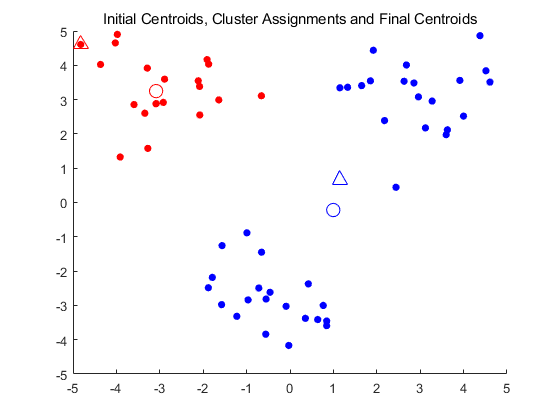
\includegraphics[width=\linewidth]{images/res23}
	\end{minipage}
	\begin{minipage}{0.48\linewidth}
		\centering
		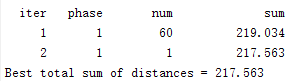
\includegraphics[width=\linewidth]{images/res231}
	\end{minipage}
	\caption{\label{res23}K=2聚类结果(曼哈顿距离作为度量)}
\end{figure}

\subsection{K=4}
同样的,我们我们选择曼哈顿距离作为度量,观察数据设计初始聚类中心为:[-4.822 4.607;-1.149 -2.493;0.232, -3.222;4.377 4.864],实验结果如图\ref{res41}所示。从图中可以看出,聚类效果还是很不错的,并且迭代两次便收敛了,收敛速度也很快。
\begin{figure}[!h]
	\centering
	\begin{minipage}{0.48\linewidth}
		\centering
		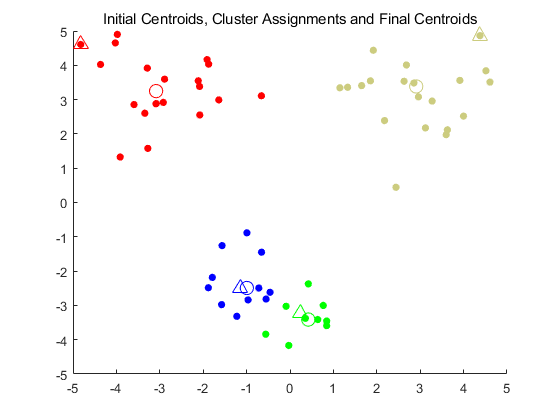
\includegraphics[width=\linewidth]{images/res41}
	\end{minipage}
	\begin{minipage}{0.48\linewidth}
		\centering
		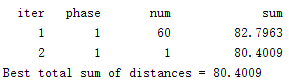
\includegraphics[width=\linewidth]{images/res42}
	\end{minipage}
	\caption{\label{res41}K=4聚类结果(曼哈顿距离作为度量)}
\end{figure}

\section{实验结论}
从结果来看,最终的聚类效果与初始条件的设置有很大的关系,因此,在聚类之前观察数据的分布,选择较好的类别数和聚类中心能够得到更好的聚类效果。

\chapter{分层聚类}
有可用高斯分布近似的两个样本集:
\begin{equation}
\begin{aligned}
\omega_1&=\{(2,0),(2,2),(2,4),(3,3)\} \\
\omega_2&=\{(0,3),(-2,2),(-1,-1),(1,-2),(3,-1)\}
\end{aligned}
\end{equation}
\begin{itemize}
	\item 求:用最小错误概率分类时的识别界面
	\item 令$\omega=\omega_1\cup\omega_2$,距离取最远距离$d_{max}(S_i,S_j)=\max\limits_{X_i\in S_i,X_j\in S_j}||X_i-X_j||$,使用分层聚类法聚类并作图。
\end{itemize}

\section{用最小错误概率分类时的识别界面}
使用最小错误概率分类算法已在上次作业中实现,因此本次直接调用了上次高斯分布时判决的函数代码进行实验。
首先计算两个类的类均值:
\begin{equation}
M_1=[2.25,2.25], M_2=[0.2,0.2]
\end{equation}

根据无偏估计的协方差矩阵计算方法:
\begin{equation}
\Sigma_i=\frac{1}{N-1}\left(\omega_i-M_i\right)^T\left(\omega_i-M_i\right)\quad i=1,2
\end{equation}

计算两个类的协方差矩阵:
\begin{equation}
\Sigma_1=\left[\begin{array}{cc}
0.25 & 0.25\\
0.25 & 2.9167
\end{array}\right],\Sigma_2=\left[\begin{array}{cc}
3.7 & -2.05 \\
-2.05 & 4.7
\end{array}\right]
\end{equation}

计算正态分布时贝叶斯判别准则所需要的参数如下:
\begin{equation}
\begin{aligned}
\mathbf{W}_1&=-\frac{1}{2}\Sigma_1^{-1}=\left[\begin{array}{cc}
-2.1875 & 0.1875 \\
0.1875 & -0.1875
\end{array}\right] \\
\mathbf{W}_2&=-\frac{1}{2}\Sigma_2^{-1}=\left[\begin{array}{cc}
-0.1782 & -0.0777 \\
-0.0777 & -0.1403
\end{array}\right] \\
\mathbf{w}_1&=\Sigma_1^{-1}M_1=[9,0]^T; \\
\mathbf{w}_2&=\Sigma_2^{-1}M_2=[0.1024,0.0872]^T; \\
w_{10}&=-\frac{1}{2}M_1^T\Sigma_1^{-1}M_1-\frac{1}{2}\ln |\Sigma_1|+\ln P(\omega_1)=-10.6154 \\
w_{20}&=-\frac{1}{2}M_2^T\Sigma_1^{-1}M_2-\frac{1}{2}\ln |\Sigma_2|+\ln P(\omega_2)=-2.0017
\end{aligned}
\end{equation}

对任意数据点$\mathbf{x}=[x_1,x_2]^T$,计算两类的识别函数如下:
\begin{equation}
\begin{aligned}
d_1(\mathbf{x})&=\mathbf{x}^T\mathbf{W}_1\mathbf{x}+\mathbf{w}_1^T\mathbf{x}+w_{10} \\
&=-2.1875x_1^2-0.1875x_2^2+9x_1-10.6154 \\
d_2(\mathbf{x})&=\mathbf{x}^T\mathbf{W}_2\mathbf{x}+\mathbf{w}_2^T\mathbf{x}+w_{20} \\
&=-0.1782x_1^2-0.1403x_2^2+0.1024x_1+0.0872x_2-2.0017
\end{aligned}
\end{equation}

则判别函数如下:
\begin{equation}
f(\mathbf{x})=\left\{\begin{array}{cc}
x\in\mbox{class1} & \mbox{if}\quad d_1(\mathbf{x})>d_2(\mathbf{x}) \\
x\in\mbox{class2} & else
\end{array}\right.
\end{equation}

计算识别界面如下:
\begin{equation}
d_1(\mathbf{x})=d_2(\mathbf{x})\Rightarrow 2.0093x_1^2+0.0472x_2^2-0.5305x_1x_2+9.1024x_1+0.0872x_2-12.6172=0
\end{equation}

由此可以看出,分类界面在此种情况下是椭圆。

绘制出两个二维高斯分布的曲面如图\ref{gauss1}所示,识别界面如图\ref{res1}所示
\begin{figure}[!h]
	\centering
	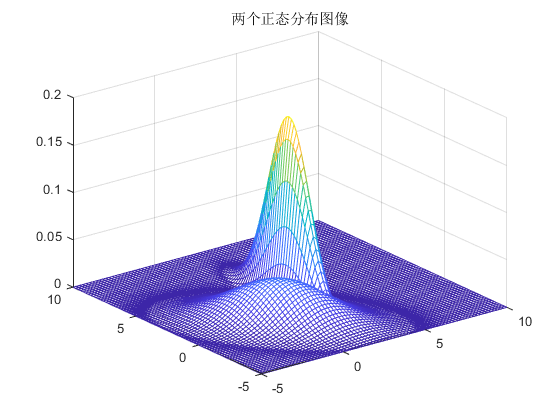
\includegraphics[width=\linewidth]{gauss1}
	\caption{\label{gauss1}二维高斯分布密度函数曲面}
\end{figure}
\begin{figure}[!h]
	\centering
	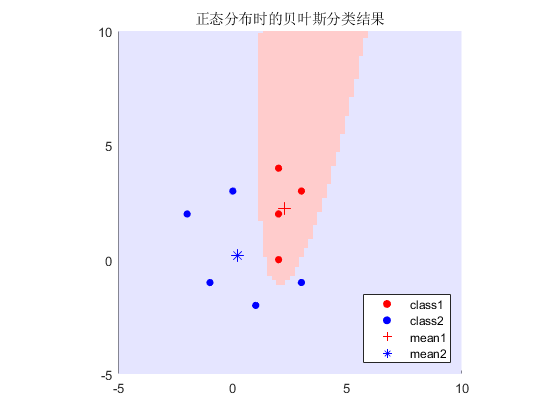
\includegraphics[width=\linewidth]{images/res1}
	\caption{\label{res1}识别界面}
\end{figure}

\newpage
\section{分层聚类}
使用最远距离作为度量,层次聚类的结果如图\ref{res5}所示,其中每层聚合图如图\ref{res6}所示。
\begin{figure}[!h]
	\centering
	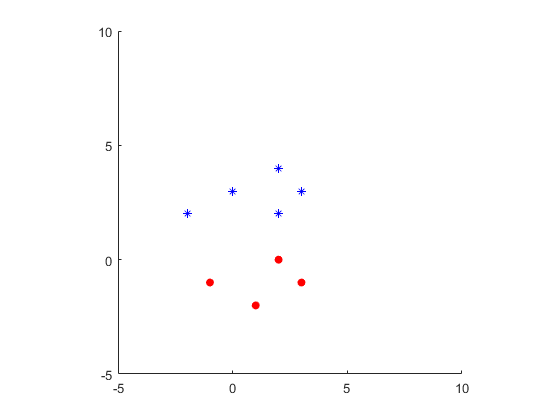
\includegraphics[width=0.89\linewidth]{hierarchical2}
	\caption{\label{res5}层次聚类结果图}
\end{figure}

\begin{figure}[!h]
	\centering
	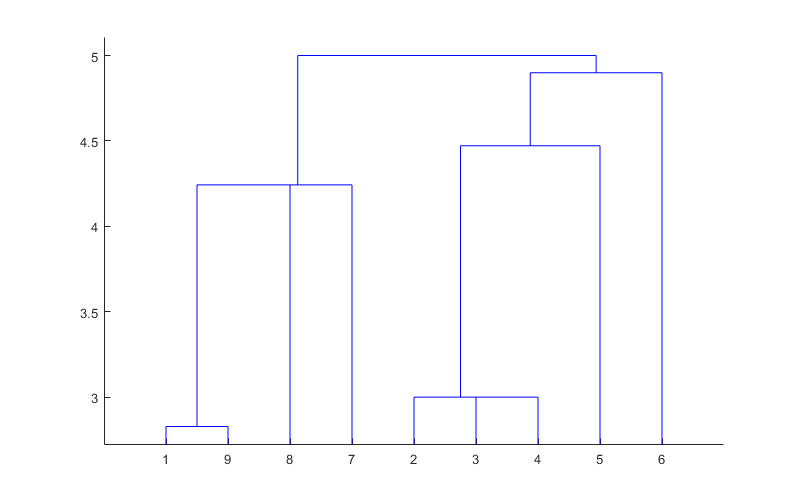
\includegraphics[width=0.89\linewidth]{hierarchical1}
	\caption{\label{res6}层次聚类树}
\end{figure}

作为对比,我们使用闵科夫斯基距离(式\ref{eq1})在不同$p$值下进行层次聚类,我们使用了$p=2,5,10,50,100$进行实验,($p=2$时为欧氏距离,$p=+\infty$时为最远距离)结果如图\ref{p2},\ref{p3},\ref{p4},\ref{p5},\ref{p6}所示,从图中可以看出,层次聚类的过程有轻微的差别,但是最终结果都是一致的。
\begin{equation}
\label{eq1}
d_{ij}=\left(\sum_{k=1}^{m}\left|x_{kj}-x_{ki}\right|^p\right)^{\frac{1}{p}}
\end{equation}

\begin{figure}[!h]
	\centering
	\begin{minipage}{0.48\linewidth}
		\centering
		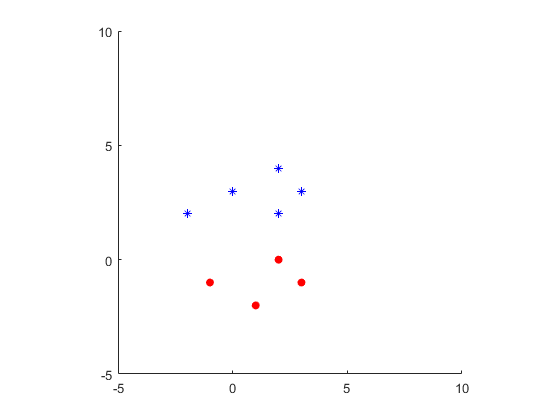
\includegraphics[width=0.89\linewidth]{hierarchical2}
	\end{minipage}
	\begin{minipage}{0.48\linewidth}
		\centering
		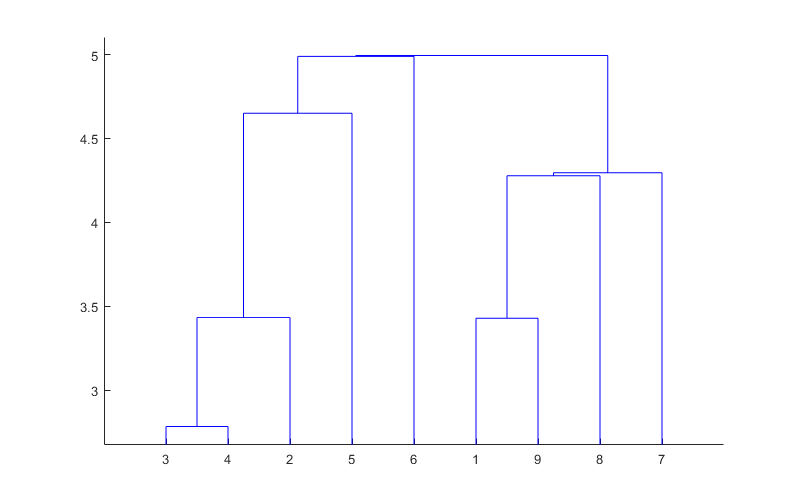
\includegraphics[width=0.89\linewidth]{p2}
	\end{minipage}
	\caption{\label{p2}p=2时聚类结果(即为欧式距离)}
\end{figure}

\begin{figure}[!h]
	\centering
	\begin{minipage}{0.48\linewidth}
		\centering
		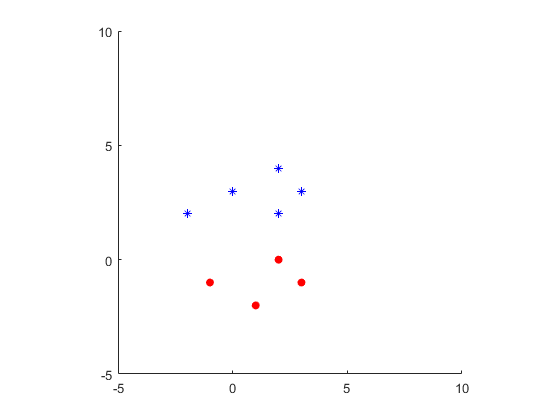
\includegraphics[width=0.89\linewidth]{hierarchical2}
	\end{minipage}
	\begin{minipage}{0.48\linewidth}
		\centering
		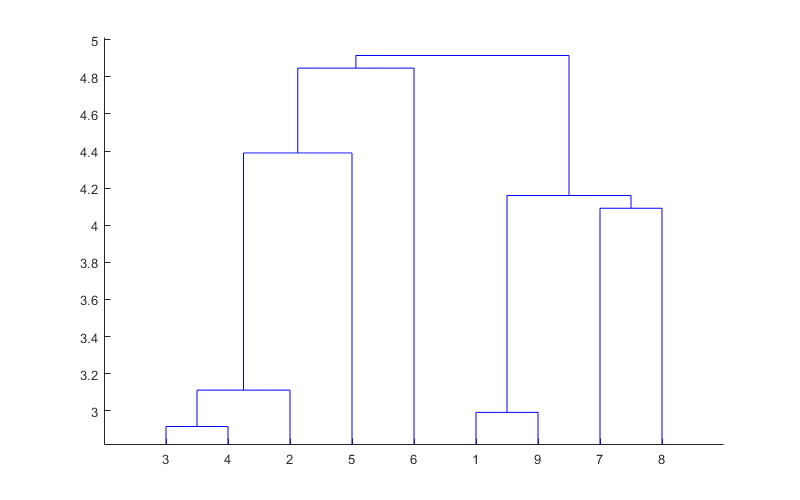
\includegraphics[width=0.89\linewidth]{p5}
	\end{minipage}
	\caption{\label{p3}p=5时聚类结果}
\end{figure}

\begin{figure}[!h]
	\centering
	\begin{minipage}{0.48\linewidth}
		\centering
		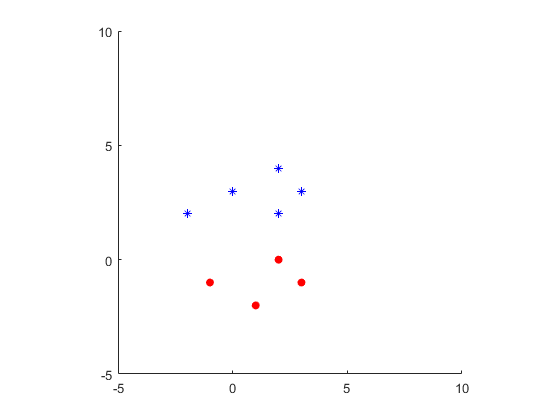
\includegraphics[width=0.89\linewidth]{hierarchical2}
	\end{minipage}
	\begin{minipage}{0.48\linewidth}
		\centering
		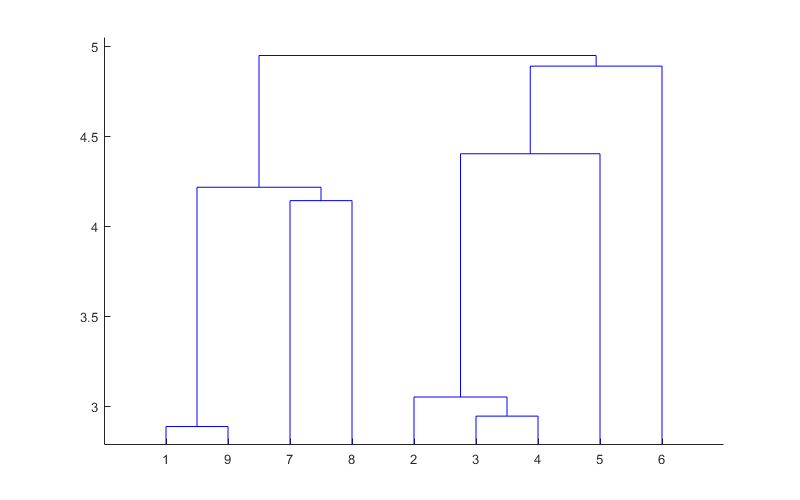
\includegraphics[width=0.89\linewidth]{p10}
	\end{minipage}
	\caption{\label{p4}p=10时聚类结果}
\end{figure}

\begin{figure}[!h]
	\centering
	\begin{minipage}{0.48\linewidth}
		\centering
		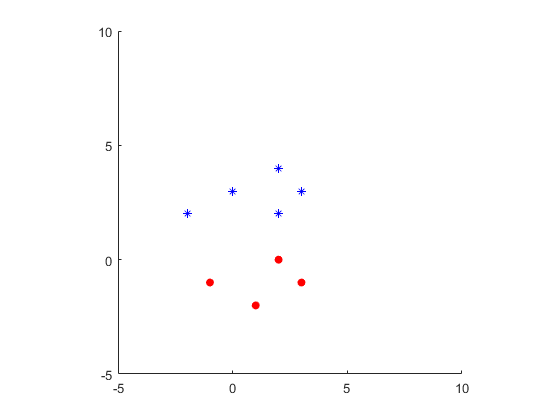
\includegraphics[width=0.89\linewidth]{hierarchical2}
	\end{minipage}
	\begin{minipage}{0.48\linewidth}
		\centering
		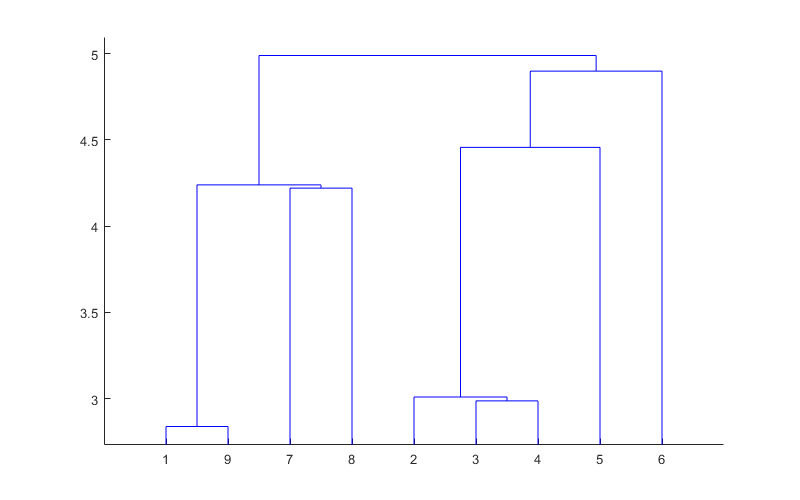
\includegraphics[width=0.89\linewidth]{p50}
	\end{minipage}
	\caption{\label{p5}p=50时聚类结果}
\end{figure}

\begin{figure}[!h]
	\centering
	\begin{minipage}{0.48\linewidth}
		\centering
		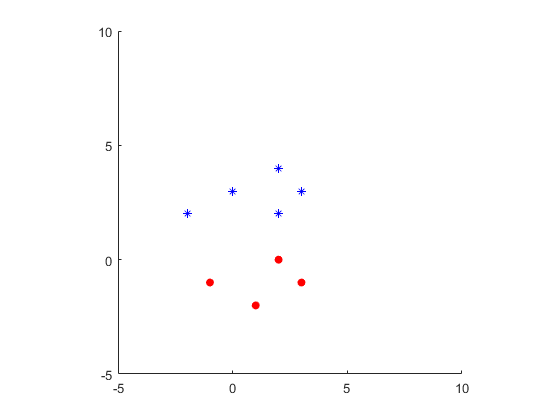
\includegraphics[width=0.89\linewidth]{hierarchical2}
	\end{minipage}
	\begin{minipage}{0.48\linewidth}
		\centering
		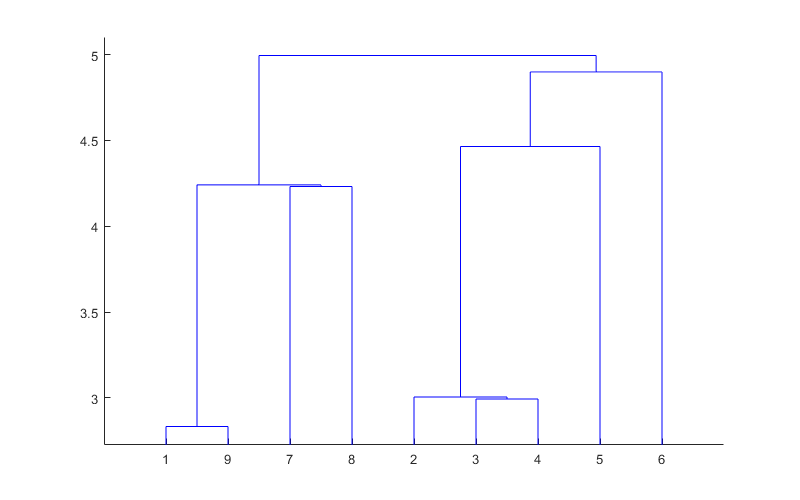
\includegraphics[width=0.89\linewidth]{p100}
	\end{minipage}
	\caption{\label{p6}p=100时聚类结果}
\end{figure}

\chapter{代码说明}
\noindent 本次实验使用Matlab语言编写,所有代码放置在“code/”文件夹下:
\begin{itemize}
	\item kmeansmain.m: 使用kmeans聚类讨论的主程序,直接执行即可;
	\item Bayes\_Gauss.m: 使用高斯分布时的贝叶斯判别准则绘制分类界面的函数,与上次作业一致;
	\item gauss\_main.m: 使用最小错误率绘制识别界面的主函数,直接执行即可;
	\item hierarchical\_cluster.m: 使用层次聚类的主程序,直接执行即可。
\end{itemize}
\end{document}